
\section{Conclusions}
%Explain what conclusions you can draw from these set of experiments? The set of experiments and results reported here should justify some of the design choices described in the previous sections. (3-6 pages)

We plot the Inception score evolution of all our models evaluated on CIFAR10 in Figure \ref{fig:exp-all-is}.
\begin{figure}[h]
\centering
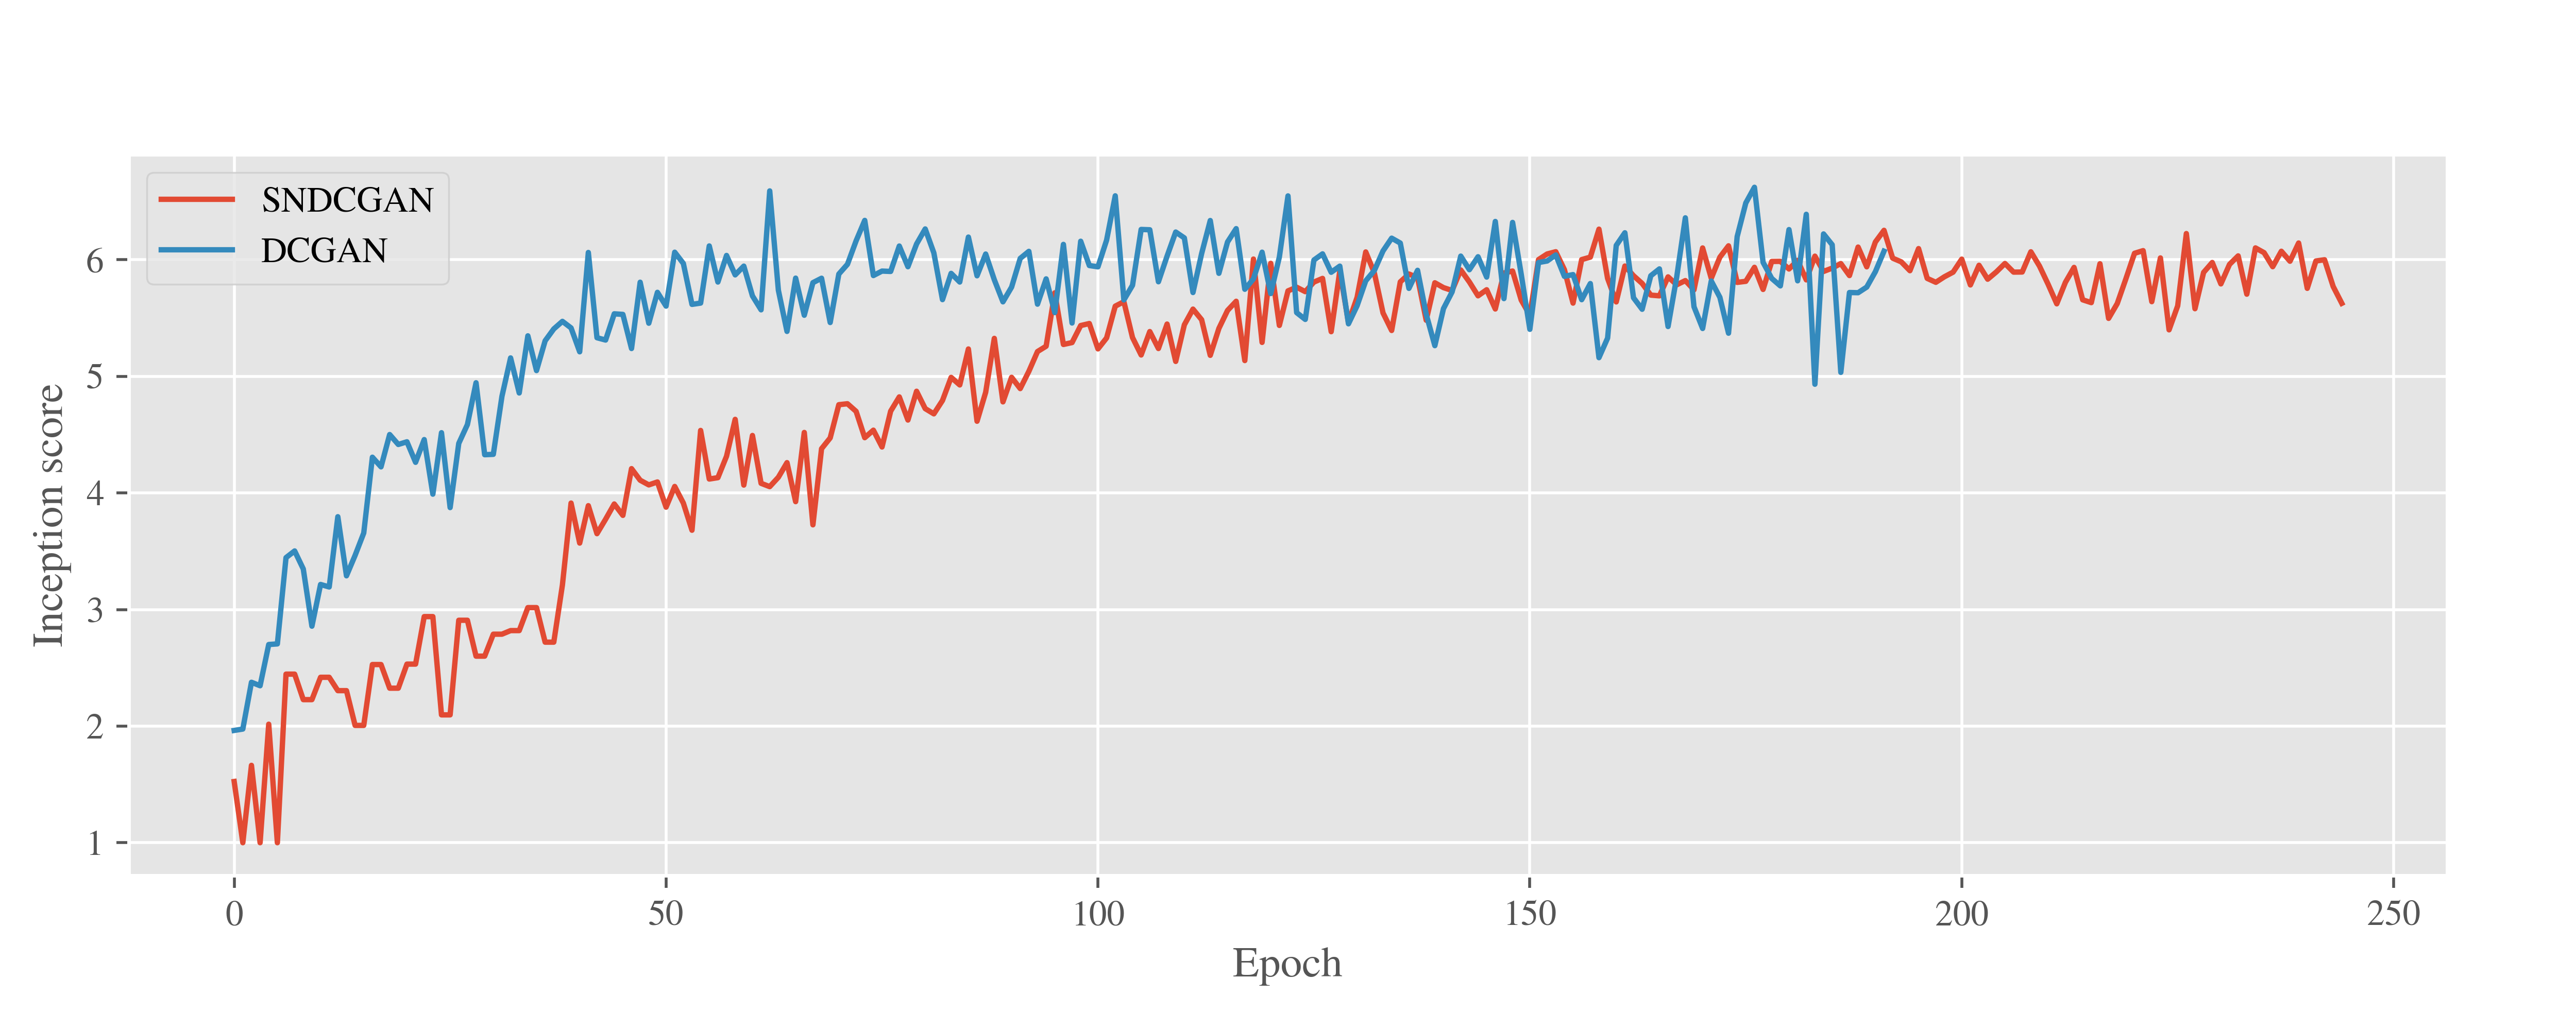
\includegraphics[width=\textwidth]{../code/results/figures/all_cifar10_is.png}
\caption{All evaluated models - Inception score, training on CIFAR10}
\label{fig:exp-all-is}
\end{figure}



\todo{to justify the use of WGAN / the need for loss smoothness: Plotting these learning curves is not only useful for debugging and hyperparameter searches, but also correlate remarkably well with the observed sample quality. (taken from WGAN paper) }

\subsection{Future Work}


- LSGAN
- Gradient penalty
- Parameter search